% ProjectTemplate.tex LaTeX template for Complexity and Networks projects
% T.S.Evans, K. Christensen Imperial College, London

\documentclass[a4paper,12pt]{article}

% These packages are standard and very useful for many mathematical symbols but you may well not need them
%\usepackage{amsmath,amssymb,amscd}

% *** FIGURES
% Info on figures at http://en.wikibooks.org/wiki/LaTeX/Floats,_Figures_and_Captions
%
% --- graphicx
\usepackage{graphicx}
\usepackage{amssymb}
% This is the main one used to read in images.  ESSENTIAL
%
% I DO NOT recommend you try anything else.  Messing around with inages in LaTeX is a pain.
% Try making an image or figure 5\% smaller in LaTeX can make all the difference



% for sub figures
\usepackage{caption}
\usepackage{subcaption}



% Change Page Size
\usepackage[a4paper,margin=2.5cm, marginparwidth=2.5cm]{geometry}



% *** HYPERLINKS
%
\usepackage{hyperref}
%
% See http://en.wikibooks.org/wiki/LaTeX/Hyperlinks
% or hyperref manual.  Main LaTeX reference systems automatically made into hyperlinks in pdf document.
% Again this should always be the last package to be defined which may cause issues with showkeys.
% An out-of-memory error might be caused by this package if its in the wrong position.
% For additional hypelinks in the text try
%   \hyperref[mainlemma]{lemma \ref*{mainlemma}}
%   \url{<my_url>}
%   \href{<my_url>}{<description>}
% Now define replacements which will work even if hyperref not included
\providecommand{\href}[2]{\texttt{#2}}
\providecommand{\url}[1]{\texttt{#1}}


% *** KEYS SHOWN IN DRAFTS
%
%\usepackage{showkeys}
%
% This is great for drafts as it will show all the labels you have defined.
% DON'T forget to comment it out before submission
% Always the last package to define.
% An out-of-memory error might be caused by this package if its in the wrong position.

% Shorthand for list environments
\providecommand{\bi}{\begin{itemize}}
\providecommand{\ei}{\end{itemize}}
\providecommand{\bd}{\begin{description}}
\providecommand{\ed}{\end{description}}
\providecommand{\ben}{\begin{enumerate}}
\providecommand{\een}{\end{enumerate}}

% Add up marks, not needed for actual reports, just for this template
\newcounter{nmarks}
\newcommand{\qmarks}[1]{\addtocounter{nmarks}{#1} }
\newcommand{\totalmarks}{}
% *** You do NOT want marks in your report so comment out the next two lines. ***
\renewcommand{\qmarks}[1]{\addtocounter{nmarks}{#1} \hspace*{\fill} [\textbf{#1~marks}]}
\renewcommand{\totalmarks}{\hspace*{\fill} [\textbf{Total~\arabic{nmarks}~marks}]}

\usepackage{physics}

% Optional, example given here for simple headers
%\pagestyle{myheadings}
%\markboth{CID: \texttt{012345678} Network Project}{CID: \texttt{012345678} Network Project}


\begin{document}

% Maybe it is just as easy to lay the title page out yourself.
% The following lines are one way to do this.
% Otherwise try \maketitle and look up associated commands for that

\begin{center}
 {\Large\textbf{Network Project}}  \\[3pt]
 {\Large\textbf{A Growing Network Model}} \\[6pt]
 % NO NAME for anonymous marking
 {\large CID: \texttt{01881584}} \\[3pt]
 17th February 2023 % Use \today or put your own date in here
\end{center}


% Abstract carries no specific marks but could be assessed as part of the overall "Professional Skills" marks
\vspace*{2cm}
\noindent
\textbf{Abstract}: You may want to write a concise abstract that briefly puts the
work into context, explains what was done, how it was done, the main results,
the conclusions you could draw and the implications.

% The Word count is part of the brief.  They carry no specific marks but could be assessed as part of the overall "Professional Skills" marks
% Excludes front page with any abstract, figure captions, table captions, acknowledgement and bibliography.
% You could use delatex to help you remove latex commands but a simple estimate
% (count words per line on several lines, count lines on every page) will do.
\vspace*{0.5cm}
\noindent
\textbf{Word Count}: \texttt{????} words excluding font page, figure captions, table captions, acknowledgement and bibliography.


% *********************************************************
%
% Everything from here to the \newpage is for your information.
% Delete this from your finished report
% You could always put a nice picture here instead.
%

%
%
% *********************************************************







% ********************************************************
\setcounter{section}{-1}
\section{Introduction}\label{sintro}

Brief paragraph with your Aims and Objectives. Marked under the ``Professional Skills'' category.

% ..............................................
\subsection*{Definition}

Give your definition of the BA model as implemented by you in this work. \qmarks{3} TOTOTO


% ********************************************************
\section{Phase 1: Pure Preferential Attachment $\Pi_\mathrm{pa}$}

% ---------------------------------------------
\subsection{Implementation}



% ..............................................
\subsubsection{Numerical Implementation}
Describe how you implemented the BA model numerically. \qmarks{3} %(2010 3 marks?)

I wrote a python class that represents a single network. It stores the adjacency list (since the network will be sparse) and an array of \textit{unnormalized probabilities}, aka weights, one entry for each vertex. First, the model initializes a network drawing from a variety of methods (even though I consistently started with random regular networks), and then simulates a number of steps. In each step, $m$ vertices are picked at random, with the selection probability being proportional to their weights, and then a vertex and $m$ edges are added to the adjacency list, updating the weights according to the specific probability strategy PS (here preferential attachement).

The random selection is done without replacement, so each pair of vertices can be connected by up to one edge. The random regular network generator \textit{de facto} keeps randomly picking from available edges until either the process is done or there is a dead end, which prompts a retry, so even though it's horrifically ineffectove, it's entirely random.

% ..............................................
\subsubsection{Initial Graph}
What type of initial graph do you use and why? \qmarks{3}

I use a random regular graph with $k_i=m$, so that $p(k<m,t)=n(k<m,t)=0\forall t$ (the \textit{lowest degree condition}). Starting with a `shapeless' $k$ distribution also prevents potential initial-value conditions altering the measurements -- for example, if we started with a graph where all $k=1$ except for $k_1=1000$, then that one vertex would be getting almost all of the new edges, highly increasing the network size $N$ required for the $k$ distribution to converge to a power law distribution.

% ..............................................
\subsubsection{Type of Graph}
What type of graph do you produce and why? \qmarks{3}

We end up with a simple, sparse network. \textbf{Simple}, because our rules don't allow self-loops or multiple edges connecting two vertices, and \textbf{sparse}, because $N(t)$ and $E(t)$ are of the same order (see proof below).

% ..............................................
\subsubsection{Working Code}
How do you know that your programme is working correctly? \qmarks{2}


% ..............................................
\subsubsection{Parameters}
Describe the parameters your programme needs, the values you chose, and why. \qmarks{2}

The network itself needs to know its probability strategy (in this section always preferential attachement `PA'), the value of $m$, the size of the initial graph $N_0$ and the size of the final graph $N_{\mathrm{final}}$. I chose $m=1, 3, 5$, since the time complexity is proportional to $m$ and, in our theoretical distribution, $m$ is just a factor and therefore not too interesting. $N_0$ I always set to $2(m+1)$ so that the regular graph is possible to create, and so that the initial size is relatively (to $N_{\mathrm{final}}$) small. I chose $N_{\mathrm{final}} = 2\cdot 10^5$, because I checked that for that size the goodness-of-fit numbers barely fluctuate for my chosen values of $m$, so we can assume they've reached their limit here.

% ---------------------------------------------
\subsection{Preferential Attachment Degree Distribution Theory}

% ..............................................
\subsubsection{Theoretical Derivation}
Give your best theoretical derivation for the form of the degree distribution $p(k)$ in the long-time limit for Preferential Attachment (PA) in the BA model. \qmarks{4}

\hfill\\
Let $t$ be the number of vertices added to the initial graph (aka time), $N(t)=N_0+t$ be the number of vertices, $E(t)=E_0 + mt$ be the number of edges, $p(k, t)$ be the probability that a random vertex has degree $k$, and $n(k, t)=N(t)p(k,t)$ be the expected number of vertices with degree $k$. Then, in each step, for each degree value $k$, the expected number of vertices with that degree that has a new edge connected to them is $m\Pi(k,t)n(k,t)$. Also, in each step, one vertex with degree $m$ is being added. Hence we can describe how the \textit{expected} number of vertices of a certain degree changes in each iteration:
\begin{equation} \label{MasterEquation}
n(k, t+1) = n(k, t) + m \left[\Pi(k-1,t)n(k-1,t) - \Pi(k,t)n(k,t)\right] + \delta_{k,m}
\end{equation}
We can express \ref{MasterEquation} with $p(k,t)$ and $N(t)$:
\begin{eqnarray*}
N(t+1)p(k, t+1) &=& N(t)p(k, t) + mN(t) \left[\Pi(k-1,t)p(k-1,t) - \Pi(k,t)p(k,t)\right] + \delta_{k,m}
\end{eqnarray*}
Consider the limit
$$\lim_{t\to\infty} p(k,t)\equiv p_\infty (k)$$
In this limit, the probability distribution function of the degrees should stay constant, and is given by the equation
\begin{equation} \label{MasterEquationLimit}
p_\infty(k) = \lim_{t\to\infty} m \left[N(t)\Pi(k-1,t)p_\infty(k-1) - N(t)\Pi(k,t)p_\infty(k)\right] + \delta_{k,m}
\end{equation}
Up until this point, the shape of $\Pi(k,t)$ could be anything. Here, to solve this equation, we apply the Preferential Attachment model, which requires $\Pi(k,t)\propto k$. Writing this as $\Pi(k,t)=c(t)k$, we now require $\Pi$ to be normalized and hence find $c(t)$:
\begin{eqnarray*}
\sum_{i\in\mathrm{vertices}} \Pi(k_i,t)&=&1\\
c(t) \sum_{i\in\mathrm{vertices}} k&=&1\\
c(t) \cdot 2E(t)&=&1\\
\Pi(k,t) &=& \frac{k}{2E(t)}
\end{eqnarray*}
Now: we want to calculate the following limit:
$$\lim_{t\to\infty}\frac{N(t)}{E(t)}=\lim_{t\to\infty}\frac{N_0+t}{E_0+mt}=\frac{1}{m}$$
Plugging these two results into \ref{MasterEquationLimit}, we obtain
\begin{equation} \label{MasterEquationLimitPA}
p_\infty(k) = \frac{1}{2}\left[(k-1)p_\infty(k-1) - kp_\infty(k)\right] + \delta_{k,m}
\end{equation}
First, we consider the case $k>m$. To solve this, we rearrange as
$$\frac{p_\infty(k)}{p_\infty(k-1)}=\frac{k-1}{k+2}$$
and note that if we make $p_\infty(k)$ proportional to $\left[k(k+1)(k+2)\right]^{-1}$, then $p_\infty(k-1)$ will be proportional to this sequence `shifted' -- ergo $p_\infty(k-1)\propto \left[(k-1)k(k+1)\right]^{-1}$ -- and their ratio is then exactly what's required. Therefore
$$p_\infty(k)=\frac{A}{k(k+1)(k+2)}\qq{when} k>m$$
Now we consider the case $k=m$. Applying the lowest degree condition yields the equation
$$p_\infty(m)=-\frac{m}{2}p_\infty(m)+1$$
Hence
$$p_\infty(m)=\frac{2}{m+2}$$
We now determine the constant $A$ by considering:
\begin{eqnarray*}
\frac{p_\infty(m+1)}{p_\infty(m)}&=&\frac{m}{m+3}\\
\frac{m+2}{2}\frac{A}{(m+1)(m+2)(m+3)}&=&\frac{m}{m+3}\\
A&=&2m(m+1)
\end{eqnarray*}
When we plug this into $p_\infty(k)$, we see that setting $k=m$ yields exactly $\frac{2}{m+2}$, so we can write the result as
\begin{equation} \label{PAprob}
p_\infty(k)=\begin{cases}
\frac{2m(m+1)}{k(k+1)(k+2)} & k\geq m\\
0 & \mathrm{otherwise}
\end{cases}
\end{equation}

% ..............................................
\subsubsection{Theoretical Checks}
Check your approximate theoretical solution for $p(k)$ has the correct properties. \qmarks{4}

\hfill\\
In our derivation of $p_\infty(k)$, we never once used the fact that it must be normalized to $1$, since it's a probability distribution function. We have to check if this is true:
\begin{eqnarray*}
\sum_{k=m}^\infty p_\infty(k) &=& 2m(m+1)\sum_{k=m}^\infty \frac{1}{k(k+1)(k+2)}\\
&=& 2m(m+1)\sum_{k=m}^\infty \left[ \frac{1}{2}\frac{1}{k} - \frac{1}{k+1} + \frac{1}{2} \frac{1}{k+2} \right]\\
&=& 2m(m+1)\left( \frac{1}{2}\left(\frac{1}{m}+\frac{1}{m+1}\right) + \sum_{k=m}^\infty \left[\frac{1}{k+2}-\frac{1}{k+1} \right] \right)
\end{eqnarray*}
We recognize that the series on the right side is telescoping, hence we have
\begin{eqnarray*}
&=&2m(m+1)\left( \frac{2m+1}{2m(m+1)} - \frac{1}{m+1} + \lim_{k\to\infty} \frac{1}{k+2} \right)\\
&=&2m(m+1)\left( \frac{1}{2m(m+1)} \right)\\
\sum_{k=m}^\infty p_\infty(k) &=&  1
\end{eqnarray*}


% ---------------------------------------------
\subsection{Preferential Attachment Degree Distribution Numerics}

% ..............................................
\subsubsection{Fat-Tail}
How did you deal with any problems that a fat-tailed distribution causes? \qmarks{4}

The fat-tailed distribution of $k$ means there will be many zero-valued entries for large $k$ that are still smaller than $k_1$. Also, since we're dealing with huge networks ($N\sim 10^5$), equally-sized bins that wouldn't lose details for small $k$ would mean we would have a large number of categories (bins). Both of these problems can be solved by log-binning: the width of each bin is equal to the width of the previous bin multiplied by some constant (which I set to $1.3$, but the statistical values don't vary by much when this value is tweaked slightly). For my goodness-of-fit tests etc, I therefore reduced the distribution dataset to a log-binned histogram.

% ..............................................
\subsubsection{Numerical Results}
Show how you compared your theoretical result to your numerical data for fixed $N$ but different $m$.
Give a visualisation which shows you whether you have a good or bad fit of your numerical data to your theoretical results.
\qmarks{4}

I ran the simulation for $N=2\cdot 10^5$ and $m=1, 3, 5$. I plotted the approximate probability density distribution and the bin counts, both agreeing with the theoretical prediction.

\begin{figure}[htb]
  \begin{center}
      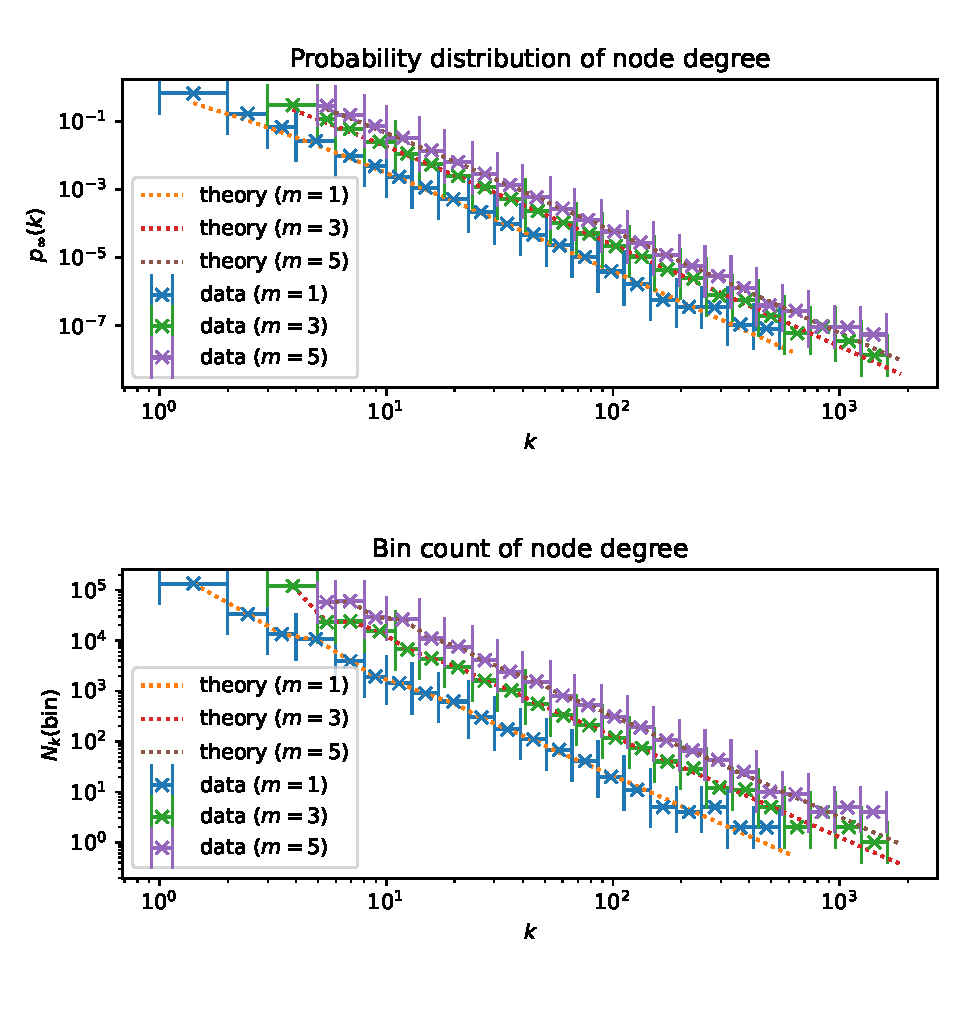
\includegraphics[width=0.7\textwidth]{images/task1_3.pdf}
  \end{center}
      \caption{Degree distribution for preferential attachement. The top plot shows the probability density distribution of $k$ approximated from the measured data by dividing the bin counts by the bin widths and then normalizing by the factor of $N^{-1}$. The bottom plot shows the raw bin counts, on which the goodness-of-fit test is done (after tail compression). We see that since all distributions resemble straight lines on a log-log plot, they are power laws.}
      \label{fig_task_1_3} %always put the label command after the caption for a figure or table.
\end{figure} 

% ..............................................
\subsubsection{Statistics}
Show statistically whether your numerical data fits your theoretical predictions. \qmarks{6}

Since I deal with binned data, I make a theoretical prediction of the count in each bin (as a partial sum of $p_\infty(k)$) and compare that to the measured values. Since I deal with categorical data, I used $\chi^2$ testing, which calculates the $\chi^2$ statistic of a dataset, which represents the `distance' of the data form the theoretical prediction, and then calculates the probability $p$ that a dataset with such $\chi^2$ statistic or higher would be measured \textit{given} the data follows the theoretical prediction. Here, $H_0$ is that the data does follow the prediction, and a large $p$ (usually taken as larger than $0.05$) means we failed to reject $H_0$, which is evidence that the fit is good.


% ---------------------------------------------
\subsection{Preferential Attachment Largest Degree and Data Collapse}


% ..............................................
\subsubsection{Largest Degree Theory}
Give your best theoretical estimate of how the largest expected degree, $k_\mathrm{1}$ (subscript 1 indicating the degree of the vertex ranked first by degree size) depends on the number of vertices $N$ in a finite size system and on $m$ the number of edges added each step. \qmarks{4}

The degree distribution of a large newtork with $N$ vertices will approximately follow the derived distribution in \ref{PAprob}, hence
$$n_N(k)\approx Np_\infty(k)$$
The largest degree $k_1$ is special in the sense that the expected amount of vertices with degree $k_1$ \textit{or higher} is $1$:
\begin{equation} \label{MaximumDegree}
N\sum_{k=k_1}^\infty p_\infty(k)=1
\end{equation}
We already know how to calculate this sum, so we evaluate:
\begin{align*}
N\sum_{k=k_1}^\infty &= 2Nm(m+1)\left[\frac{1}{2}\left(\frac{1}{k_1}+\frac{1}{k_1+1}\right)-\frac{1}{k_1+1}\right]\\
&=Nm(m+1)\frac{1}{k_1(k_1+1)}\\
k_1^2+k_1 &= Nm(m+1)\\
k_1 &= \frac{-1\pm\sqrt{1+4Nm(m+1)}}{2}
\end{align*}
$k_1$ cannot be negative, hence we take the positive root:
\begin{equation} \label{MaximumDegreePA}
k_1 = \frac{-1+\sqrt{1+4Nm(m+1)}}{2}
\end{equation}

% ..............................................
\subsubsection{Numerical Results for Largest Degree}
Study of the behaviour of $k_1$ as $N$ is varied for one sensible fixed value of $m$ (justify your choice of parameters). Estimate uncertainties/errors where possible. Compare against your theoretical prediction. \qmarks{4}

% ..............................................
\subsubsection{Data Collapse}
Illustrate the finite size effects by studying a single value of $m$ (justify your choice for $m$) but varying $N$ and looking for data collapse. You should describe how you tried to use an understanding of the $k_1$ scale to look for any finite size effects in the tail of the distribution, describing any results found. Further mathematical investigation of finite size effects is not required as it is extremely hard to do. \qmarks{4}

The existence of $k_1(N)$ means that a network of size $N$ will experience a cut-off in its degree distribution around $k=k_1$. We use the following ansatz to describe this finite-size effect:
\begin{equation} \label{FiniteSizeAnsatz}
p_N(k)=p_\infty(k)\mathcal{F}\left(\frac{k}{k_1}\right)
\end{equation}
In our data collapse, we separate $\mathcal{F}$ like so:
$$\mathcal{F}\left(\frac{k}{k_1}\right)=\frac{p_N(k)}{p_\infty(k)}=\frac{k(k+1)(k+2)}{A}p_N(k)$$
and plot it against $k/k_1$ (so we divide the x-axis by $k_1$). $p_N(k)$ here represents the actual measured values for the distribution on a network of a specific size.


% ***********************************************************************
\section{Phase 2: Pure Random Attachment $\Pi_\mathrm{rnd}$}

%%%\textbf{FOR 2023, MAKE PROMPTS/MARK SCHEME CLEARER THAT WE WANT EVERY TASK IN PHASE 1 REPEATED}


% ---------------------------------------------
\subsection{Random Attachment Theoretical Derivations}


% ..............................................
\subsubsection{Degree Distribution Theory}
Give your best theoretical derivation for the form of the degree distribution in the long-time limit. Check your approximate theoretical solution has the correct properties. \qmarks{4}

\hfill\\
For this model, we can use the same equation \ref{MasterEquationLimit} as for preferential attachment, we'll just use different $\Pi(k,t)$. Namely, in the random attachment model, every vertex has the same selection probability as any other. Hence
$$\Pi_{\mathrm{RA}}(k,t)=\frac{1}{N(t)}$$
This means our governing equation is
\begin{equation} \label{MasterEquationLimitRA}
p_\infty(k)= m\left[ p_\infty(k-1)-p_\infty(k) \right] + \delta_{k,m}
\end{equation}
Hence for $k=m$, using the lowest degree condition:
$$p_\infty(m)=\frac{1}{1+m}$$
And for $k>m$:
$$p_\infty(k)=\frac{m}{m+1}p_\infty(k-1)$$
By induction, we obtain
$$p_\infty(k)=\left(\frac{m}{m+1}\right)^{k-m}p_\infty(m)=\frac{1}{m+1}\left(\frac{m}{m+1}\right)^{k-m}$$
Hence the degree probability distribution function in this model is
\begin{equation} \label{RAprob}
p_\infty(k)=\begin{cases}
\frac{1}{m+1}\left(\frac{m}{m+1}\right)^{k-m} & k\geq m\\
0 & \mathrm{otherwise}
\end{cases}
\end{equation}
We need to check if this is normalized:
\begin{eqnarray*}
\sum_{k=m}^\infty p_\infty(k)&=&\frac{1}{m+1} \sum_{k=m}^\infty \left(\frac{m}{m+1}\right)^{k-m}\\
&=&\frac{1}{m+1} \sum_{x=0}^\infty \left(\frac{m}{m+1}\right)^x\\
&=&\frac{1}{m+1} \cdot \frac{1}{1-\frac{m}{m+1}}\\
&=& 1
\end{eqnarray*}
Therefore $p_\infty(k)$ is normalized. We see that, rather than a power law like in the preferential attachment model, the probability distribution for the random attachement model is governed by exponential decay.

% ..............................................
\subsubsection{Largest Degree Theory}
Give your best theoretical estimate of how the largest expected degree, $k_\mathrm{1}$ 
%(subscript 1 indicating the degree of the vertex ranked first by degree size) 
depends on the number of vertices $N$ in a finite size system. \qmarks{2}

By substituing \ref{RAprob} into \ref{MaximumDegree} we obtain:
\begin{align*}
1 &= N\sum_{k=k_1}^\infty \frac{1}{m+1}\left(\frac{m}{m+1}\right)^{k-m}\\
&= N\left(\frac{m}{m+1}\right)^{k_1-m}\sum_{k=m}^\infty \frac{1}{m+1}\left(\frac{m}{m+1}\right)^{k-m}\\
&= N\left(\frac{m}{m+1}\right)^{k_1-m}\\
N &= \left(\frac{m+1}{m}\right)^{k_1-m}\\
k_1 &= m+\frac{\ln{N}}{\ln(\frac{m+1}{m})}
\end{align*}

% ---------------------------------------------
\subsection{Random Attachment Numerical Results}

% ..............................................
\subsubsection{Degree Distribution Numerical Results}
Show how you compared your theoretical result to your numerical data for different $m$ at one large value of $N$.  Is your theory a good fit to your data? How did you arrive at your conclusion?  \qmarks{6}

% ..............................................
\subsubsection{Largest Degree Numerical Results}
Study of the behaviour of $k_1$ as $N$ is varied for one sensible fixed value of $m$ (justify your choice of parameters) including estimates of uncertainties on any measurements. Compare against your theoretical prediction. Illustrate the finite size effects by looking for possible data collapse.
\qmarks{4}




%%%% ****************************************************************
%%%\section{Phase 3: Mixed Preferential and Random Attachment}
%%%
%%%% ---------------------------------------------
%%%\subsection{Mixed Attachment Model Theoretical Derivations}
%%%
%%%Give your best theoretical derivation for the form of the degree distribution in the long-time limit for the specific scenario given, namely where some edges added with preferential attachment and some use random attachment. Check your solution. \qmarks{6}
%%%
%%%% ---------------------------------------------
%%%\subsection{Mixed Attachment Model Numerical Results}
%%%
%%%Explain how you compared your theoretical result to your data.  Is it a good fit and how did you arrive at your conclusion about the fit? \qmarks{6}





%%%% .................................................................
%%%\section{Phase 3: Random Walks and Preferential Attachment}\label{s:phase3}
%%%
%%%% ..............................................
%%%\subsection{Implementation}
%%%
%%%Define the model you implemented, how it was implemented and explain any choices you made. \qmarks{4}
%%%% ..............................................
%%%\subsection{Numerical results}
%%%
%%%Describe your observations of the degree distribution as best you can e.g.\ visual illustrations, quantitative information. \qmarks{6}
%%%
%%%% ..............................................
%%%\subsection{Discussion of Results}
%%%
%%%Interpret your results in terms of the mechanisms behind the emergence of large tailed degree distributions in real world networks. \qmarks{2}



% ****************************************************************
\section{Phase 3: Existing Vertices Model}

%\textbf{FOR 2022, MAKE PROMPTS/MARK SCHEME CLEARER IF WE WANT EVERY TASK IN PHASE 1 REPEATED}


% ---------------------------------------------
\subsection{Existing Vertices Model Theoretical Derivations}

Give your best theoretical derivation for the form of the degree distribution in the long-time limit for the specific scenario given, namely where some edges added run between exiting vertices while the rest are between the new vertex and one existing vertex as before. Check your solution. \qmarks{8}

\hfill\\
Here, we need to alter the equation \ref{MasterEquation}, since there are more ways the number of vertices with a specific edge can change. Namely, in each step, $r$ edges are added to the system from the new vertex to $r$ existing vertices using PDF $\Pi_1(k,t)$ and $(m-r)$ edges are added between existing vertices using PDF $\Pi_2(k,t)$. The first part can be interpreted the same way as the previous two models, with the number of vertices with changing $k$ being $r$ rather than $m$; the second part can be as well, except the number of vertices changing $k$ is $2(m-r)$, and there will be no Kronecker delta term, since no new vertex is being added. Hence the new governing equation is
\begin{multline} \label{MasterEquationEVM}
n(k,t+1)= n(k,t)+r\left[\Pi_1(k-1,t)n(k-1,t)-\Pi_1(k,t)n(k,t)\right] \\
+2(m-r)\left[\Pi_2(k-1,t)n(k-1,t)-\Pi_2(k,t)n(k,t)\right]+\delta_{r,k}
\end{multline}
We can take the limit $t\to\infty$ and express \ref{MasterEquationEVM} with $p_\infty(k)$:
\begin{multline} \label{MasterEquationEVMlimit}
p_\infty(k)=\lim_{t\to\infty}N(t)\left[2(m-r)\Pi_2(k-1,t)+r\Pi_1(k-1,t)\right]p_\infty(k-1)\\
-N(t)\left[2(m-r)\Pi_2(k,t)+r\Pi_1(k,t)\right]p_\infty(k)+\delta_{r,k}
\end{multline}
Note that since the vertices we're adding begin with degree $r$ rather than $m$, the lowest degree condition here states that $p(k<r,t)=0$.

We apply the specific shapes of $\Pi_1(k,t)=\Pi_{\mathrm{ra}}(k,t)=1/N(t),\Pi_2(k,t)=\Pi_{\mathrm{pa}}(k,t)=k/(2mN(t))$ and rearrange:
\begin{align*}
p_\infty(k)&=\left[\frac{m-r}{m}(k-1)+r\right]p_\infty(k-1)-\left[\frac{m-r}{m}k+r\right]p_\infty(k)\\
\left[1+r+\frac{m-r}{m}k\right]p_\infty(k)&= \left[r-\frac{m-r}{m}+\frac{m-r}{m}k\right]p_\infty(k-1)+\delta_{r,k}
\end{align*}
For $k=r$:
\begin{equation*}
p_\infty(r)=\frac{1}{1+r+\frac{m-r}{m}r}=\frac{m}{2mr+m-r^2}
\end{equation*}
For $k>r$:
\begin{equation*}
\frac{p_\infty(k)}{p_\infty(k-1)}=\frac{k+\frac{mr+r-m}{m-r}}{k+\frac{mr+m}{m-r}}
\end{equation*}
To solve this equation, we generalize our approach for the PA model and note that for a function $f(x)=A\Gamma(x+1+a)/\Gamma(x+1+b)$, we have
$$\frac{f(x)}{f(x-1)}=\frac{\Gamma(x+1+a)\Gamma(x+b)}{\Gamma(x+a)\Gamma(x+1+b)}=\frac{(x+a)\Gamma(x+a)}{\Gamma(x+a)}\frac{\Gamma(x+b)}{(x+b)\Gamma(x+b)}=\frac{x+a}{x+b}$$
Identifying $x\equiv k, a\equiv \frac{mr+r-m}{m-r}, b\equiv \frac{mr+m}{m-r}$ we obtain
\begin{equation*}
p_\infty(k>r)=A\frac{\Gamma(k+1+\frac{mr+r-m}{m-r})}{\Gamma(k+1+\frac{mr+m}{m-r})}=A\frac{\Gamma(k+z_1)}{\Gamma(k+z_2)}\mbox{ where }z_1=\frac{mr}{m-r},z_2=\frac{mr+2m-r}{m-r}
\end{equation*}
Now:
\begin{align*}
\frac{p_\infty(r+1)}{p_\infty(r)}&= \frac{(m-r)(r+1)+mr-m+r}{(m-r)(r+1)+mr+m} = A\frac{\Gamma(r+1+z_1)}{\Gamma(r+1+z_2)}\frac{2mr+m-r^2}{m}\\
A&= \frac{mr}{(r+1)(2mr+m-r^2)}\frac{\Gamma(r+1+z_2)}{\Gamma(r+1+z_1)}
\end{align*}
We can check whether this is normalized: we want all the probabilities to sum up to $1$. By induction, we can find the partial sum:
\begin{multline} \label{RAPApartial}
\sum_{k=k_{\mathrm{min}}>r}^{k_{\mathrm{max}}}p_\infty(k)=A\left[\frac{\Gamma(z_1+k_{\mathrm{min}})}{\Gamma(z_2+k_{\mathrm{min}})}\left(1+r+k_{\mathrm{min}}\left(1-\frac{r}{m}\right)\right)+\right.\\
\left.\frac{\Gamma(z_1+1+k_{\mathrm{max}})}{\Gamma(z_2+1+k_{\mathrm{max}})}\left(\frac{r}{m}-r-2+k_{\mathrm{max}}\left(\frac{r}{m}-1\right)\right)\right]
\end{multline}
The gamma fraction in the second term goes like $(k_{\mathrm{max}}+1)^{z_1-z_2}=(k_{\mathrm{max}}+1)^{-\frac{2m-r}{m-r}}$, so the sum converges if $-\frac{2m-r}{m-r}<-1\Leftrightarrow m>0,m>r$, which we can automatically assume to be satisfied. Hence:
\begin{align*}
\sum_{k=r}^\infty p_\infty(k) &= \frac{m}{2mr+m-r^2} + A\frac{\Gamma(z_1+r+1)}{\Gamma(z_2+r+1)}\frac{(r+1)(2m-r)}{m}\\
&= \frac{m}{2mr+m-r^2} + \frac{(2m-r)r}{2mr+m-r^2} = 1
\end{align*}
So $p_\infty(k)$ is normalized and looks like so:
\begin{equation} \label{RAPAprob}
p_\infty(k) = \begin{cases}
\frac{m}{2mr+m-r^2} & k=r\\
\frac{mr}{(r+1)(2mr+m-r^2)}\frac{\Gamma(r+1+z_2)}{\Gamma(r+1+z_1)}\frac{\Gamma(k+z_1)}{\Gamma(k+z_2)} & k>r\\
0 & \mathrm{otherwise}
\end{cases}
\end{equation}

\textbf{Maximum Degree}

To find $k_1$, we cannot solve \ref{MaximumDegree} directly, but by approximating \ref{MasterEquationEVMlimit} for countinuous $k$, expressing it as a differential equation and interpreting the Kronecker delta as a Dirac delta, so that we can apply the Green's function condition, we can approximate $p_\infty(k)$ as
\begin{equation*}
p_\infty(k)\approx \frac{m}{m-r}\left(r\frac{2m-r}{m-r}\right)^{\frac{m}{m-r}}\left(k+\frac{rm}{m-r}\right)^{-\frac{2m-r}{m-r}}
\end{equation*}
which we can put into \ref{MaximumDegree} and obtain
\begin{equation} \label{MaximumDegreeEVM}
k_1\approx \frac{(2m-r)rN^{\frac{m-r}{m}}-rm}{m-r}
\end{equation}

% ---------------------------------------------
\subsection{Existing Vertices Model Numerical Results}

Show how you compared your theoretical result to your numerical data for different $m$ at one large value of $N$.  Is your theory a good fit to your data? How did you arrive at your conclusion?  
Analyse the finite size effects by looking for possible data collapse. 
\qmarks{8}

% ********************************************************
\section{Conclusions}\label{sconcl}

Just one or two sentences to round off the report. Marked under the ``Professional Skills'' category.



% *********************************************************
%
% Delete this fbox from your finished report
%

\vspace*{1cm}
\fbox{
  \parbox{0.9\textwidth}{
    \emph{Delete text in this box from your final version.}

    \vspace*{12pt}
    \noindent
    \textbf{Note}: \emph{The Acknowledgement and Bibliography do not count towards the 2500 word limit nor the 16 page limit. An acknowledgement section is not required. For a report of this type and size, references may well not be needed but if you do reference other work, such as a useful book \cite{KN05} or a useful result \cite{E23},  a formal bibliography is one way to do this. No formal marks for either of these sections but they could be considered as part of the overall Organisation, Presentation or English marks.}
    \vspace*{12pt}
  } % end of parbox
} % end of fbox

%
%
% *********************************************************


% ********************************************************************
%\newpage


\section*{Acknowledgements}

Optional. Not required but you might want to thank A.Demonstrator or A.Friend for help.


% *****************************************************************
%
% BIBLIOGRAPHY
%
% **************************************************************
% 1) DO NOT WASTE TIME WITH BibTeX unless you REALLY KNOW WHAT YOU ARE DOING.
%    Just write it by hand.
% 2) NO bibliography is really needed for the projects
%    but you might cite something you read or which provided an image.
% 3) If we can get the item from the information you provided then it is fine.
%    The exact format is not important, but a consistent format is important.
%    Copy the style form one publication.
%    If space not an issue, titles of papers are useful.

\begin{thebibliography}{99}
\bibitem{KN05}
  K.Christensen and N.Maloney,
  \emph{Complexity and Criticality},
  Imperial College Press, London, 2005.
\end{thebibliography}


% *********************************************************
%
% Everything from here to the \newpage is for your information.
% Delete this from your finished report
%
\vspace*{2cm}

\fbox{
  \parbox{0.9\textwidth}{
    \emph{Delete text in this box from your final version.}

    \vspace*{12pt}
    \noindent
    \textbf{Professional Skills}

    \emph{Do not include this section in your report, it is for your information only}

    Your report should be
    \bi
    \item written in clear comprehensible English \qmarks{6}
    \item be well presented \qmarks{6}
    \item well organised and follows brief \qmarks{6}
    \ei
    This is highly subjective but generally most reports score well on these aspects. Many of the problems come from plots which might have: small unreadable fonts used for labels, labels used for variables are different from those in the text (they reflect the naming scheme used in the programme), unexplained equations of some fit with unrealistic accuracy in unexplained coefficients.


    \vspace*{12pt}
  } % end of parbox
} % end of fbox

%
%
% *********************************************************

\vspace*{12pt}
\totalmarks

\end{document}
